\documentclass[12pt]{article}
\usepackage[T1]{fontenc}
\usepackage{calc}
\usepackage{setspace}
\usepackage{multicol}
\usepackage{fancyheadings}
\usepackage{grffile}

\usepackage{graphicx}
\usepackage{color}
\usepackage{rotating}
\usepackage{harvard}
\usepackage{aer}
\usepackage{aertt}
\usepackage{verbatim}
\usepackage{array}
\usepackage{multirow}

\setlength{\voffset}{-0.25in}
\setlength{\topmargin}{0pt}
\setlength{\hoffset}{0pt}
\setlength{\oddsidemargin}{0pt}
\setlength{\headheight}{0pt}
\setlength{\headsep}{.4in}
\setlength{\marginparsep}{0pt}
\setlength{\marginparwidth}{0pt}
\setlength{\marginparpush}{0pt}
\setlength{\footskip}{.1in}
\setlength{\textwidth}{6.5in}
\setlength{\textheight}{9.25in}
\setlength{\parskip}{0pc}

\renewcommand{\baselinestretch}{1.5}

\newcommand{\bi}{\begin{itemize}}
\newcommand{\ei}{\end{itemize}}
\newcommand{\be}{\begin{enumerate}}
\newcommand{\ee}{\end{enumerate}}
\newcommand{\bd}{\begin{description}}
\newcommand{\ed}{\end{description}}
\newcommand{\prbf}[1]{\textbf{#1}}
\newcommand{\prit}[1]{\textit{#1}}
\newcommand{\beq}{\begin{equation}}
\newcommand{\eeq}{\end{equation}}
\newcommand{\bdm}{\begin{displaymath}}
\newcommand{\edm}{\end{displaymath}}
\newcommand{\script}[1]{\begin{cal}#1\end{cal}}
\newcommand{\citee}[1]{\citename{#1} (\citeyear{#1})}
\newcommand{\h}[1]{\hat{#1}}
\newcommand{\ds}{\displaystyle}
\newcommand{\normal}{\mathcal{N}}
\newcommand{\app}
{
\appendix
}

%\newcommand{\appsection}[1]
%{
%\let\oldthesection\thesection
%\renewcommand{\thesection}{Appendix \oldthesection}
%\section{#1}\let\thesection\oldthesection
%\renewcommand{\theequation}{\thesection\arabic{equation}}
%\setcounter{equation}{0}
%}

\newcommand{\appsection}[1]
{
\section{#1}
\renewcommand{\theequation}{\thesection\arabic{equation}}
\setcounter{equation}{0}
}


%\pagestyle{empty}
\pagestyle{fancyplain}
\lhead{}
\chead{Fiscal Policy Impacts with Adaptive Expectations}
\rhead{\thepage}
\lfoot{}
\cfoot{}
\rfoot{}

\begin{document}

\begin{titlepage}
\begin{singlespace}
\title{Fiscal Policy Impacts with Adaptive Expectations}
\date{\today}
\author{
James Murray\footnote{\textit{Mailing address}: 1725 State St., La Crosse, WI  54601. \textit{Phone}: (608)406-4068.\newline  \textit{E-mail}: jmurray@uwlax.edu.}\\Department of Economics\\University of Wisconsin - La Crosse
}

\maketitle

\thispagestyle{empty}

\abstract{This paper investigates the impact of fiscal policy on output and unemployment, specifically when fiscal policy changes are expected versus unexpected.  Market participants' understanding of the conduct of fiscal policy is modeled with a least-squares adaptive-expectations framework, where agents forecast fiscal policy variables taxes and government spending using macroeconomic variables and previous realization of fiscal variables.  Actual fiscal policy is decomposed into its predicted and unexpected components.  The impact of fiscal policy on output and unemployment is estimated with a structural vector-autoregression.}\\

\noindent \textit{Keywords}: Fiscal policy, multiplier, adaptive expectations, learning, vector autoregression. \\
\noindent \textit{JEL classification}: E31, E32, E62.
\end{singlespace}
\end{titlepage}

\section{Introduction}

TODO!

\section{Baseline Model}

Before proceeding to model agents' expectations of fiscal policy and decomposing fiscal policy into its expected and unexpected components, I present in this section a baseline structural vector autoregression model that illustrates the predicted impact of fiscal policy before considering its decomposition. 

\subsection{Data}
In this paper, I focus on two fiscal policy policy variables: government spending and taxes net of transfers.  Government spending is defined as \textit{Current Government Consumption Expenditures} plus \textit{Current Gross Government Investment Expenditures} as reported by the Bureau of Economic Analysis (BEA), and is transformed into its real value per capita using the associated price index for government consumption expenditures and gross investment and the U.S. population.  Taxes are defined as the sum of \textit{Current Tax Receipts}, \textit{Contributions to Government Social Insurance}, and \textit{Current Transfer Receipts}, less \textit{Current Transfer Payments}.  Taxes are transformed into a real value using the price index for GDP and expressed in per-capita terms.

I examine the effect of fiscal policy on the following macroeconomic outcomes: consumption, investment, GDP, and unemployment.  Data for GDP, its components, and the associated price levels come from the BEA, and are again transformed into real values per capita.  The unemployment rate is the \textit{Civilian Unemployment Rate} from the Bureau of Labor Statistics. 

 With the exception of the unemployment rate, I take the natural log of each of the above variables and remove a linear (in logs) trend.  The sample includes quarterly data on all the above variables from 1964:Q3 through 2007:Q2.

\subsection{Structural Vector Autoregression}\label{s:svar1}

Let $x_t$ denote the following vector of endogenous variables,
\bdm x_t = \left[ \begin{array}{c} y_t \\ c_t \\ i_t \\ u_t \\ t_t \\ g_t \end{array} \right] 
         = \left[ \begin{array}{c} \mbox{(Log) Real GDP per capita} \\ \mbox{(Log) Consumption per capita} \\ \mbox{(Log) Investment per capita} \\ 
             \mbox{Unemployment Rate} \\ \mbox{(Log) Taxes net of transfers per capita} \\ \mbox{(Log) Government spending per capita} \end{array} \right],
\edm
and consider a structural vector autoregression of the form,
\beq A_0 x_t = A(L) x_t + z_t, \eeq
where matrix $A_0$ describes the contemporaneous relationships between the endogenous variables, A(L) is a distributed lag polynomial, and $z_t$ is a vector of independently distributed shocks, where each row is a shock to the endogenous variable in the corresponding row in $x_t$.  

Restrictions must be placed on $A_0$ in order to identify the impacts of the i.i.d. shocks in $z_t$.  There is hardly a consensus in macroeconometrics literature using vector autoregressions on how this should be done.  \citee{hebous2010} provides an overview of four popular approaches in the fiscal policy literature, and \citee{perotti2007} provides a more detailed analysis.  Popular approaches include a Cholesky ordering of the variables, which assumes an ordering where one variable can contemporaneously affect the variables follow after it, but the reverse causation is not possible, thereby imposing zero restrictions in $A_0$.  Other strategies involve imposing calibrations on one or more parameters in $A_0$ based on prior information, such as the output elasticity on taxes.\footnote{See \citee{perotti2007}.}  Finally others impose restrictions based on estimated impulse response functions.

I identify the model by imposing a number of zero restrictions in $A_0$ that dictate directions for contemporaneous causation in the endogenous variables.  For one such restriction, I suppose that discretionary government spending is subject to a recognition lag, a decision lag, and/or an implementation lag.  This is to say that government spending decisions cannot recognize and act on economic problems quickly, and so government spending does not depend contemporaneously on macroeconomic variables, but realizations at least one quarter in the past.

Unlike government spending, I do allow for taxes, net of transfers, to depend contemporaneously on output and unemployment.  Unlike government spending, many components of net taxes are ``automatic stabilizers'' that adjust by construction to current macroeconomic conditions.  When there is an increase in unemployment, transfer payments to unemployed persons increase; when there is a decrease in taxable income, and therefore real GDP, total tax receipts fall.

I limit the extent to which the fiscal policy variables directly cause contemporaneous macroeconomic outcomes.  I suppose government spending does influence consumption and investment decisions.  Also, government spending directly influences GDP since government spending is one its components.  However, I do not allow for government spending to directly influence unemployment in the same period.  I suppose taxes directly affect only consumption and investment decisions, but they does not directly affect contemporaneous real GDP.  I let taxes influence real GDP only indirectly by allowing real GDP to be influenced contemporaneously by its components, consumption and investment.  

I suppose unemployment is slow to adjust, and so it does not respond automatically to any of the variables.  Rather I allow unemployment to contemporaneously affect consumption decisions, investment decisions, and real GDP.  Finally, I allow taxes to respond to changes in government spending, but not vice versa.\footnote{Neither the magnitudes nor meaning of the results are significantly altered by this last ordering.}

The above restrictions on causation imply the following structure for the vector autoregression,
\beq \label{eq:svar} \left[ \begin{array}{cccccc} 
     1 & a_{y,c} & a_{y,i} & a_{y,u} & 0 & a_{y,g} \\
     0 & 1 & 0 & a_{c,u} & a_{c,t} & a_{g,t} \\ 
     0 & 0 & 1 & a_{i,u} & a_{i,t} & a_{g,t} \\
     0 & 0 & 0 & 1 & 0 & 0 \\
     a_{t,y} & 0 & 0 & a_{t,u} & 1 & a_{t,g} \\
     0 & 0 & 0 & 0 & 0 & 1 \\ \end{array} \right]~ 
     \left[ \begin{array}{c} y_t \\ c_t \\ i_t \\ u_t \\ t_t \\ g_t \end{array} \right]  = 
     A(L) \left[ \begin{array}{c} y_{t-1} \\ c_{t-1} \\ i_{t-1} \\ u_{t-1} \\ t_{t-1} \\ g_{t-1} \end{array} \right] +
     \left[ \begin{array}{c} z_{y,t} \\ z_{c,t} \\ z_{i,t} \\ z_{u,t} \\ z_{t,t} \\ z_{g,t} \end{array} \right],
\eeq 
where $z_{t}$ is a vector of independently and identically distributed shocks to the endogenous variables.  I estimate equation (\ref{eq:svar}) with one lag in A(L).  Figure \ref{fg:irf} shows the estimated impulse response functions for a shock to government spending and taxes.  The results show that a positive shock to government spending leads to a statistically significant increase in consumption and real GDP, and a statistically significant decrease in unemployment.  The point estimates for the impulse response to investment suggests investment increases in response to government spending, but the response is not statistically significantly different from zero over any part of the time horizon.  In response to an increase in net taxes, consumption and investment decrease as expected, but the results are not statistically significant.  An increase in taxes causes unemployment to increase, and the response is statistically significantly above zero over part of the time horizon.  Strangely, the impulse response function for real GDP to a tax shock suggests an increase in taxes initially causes real GDP to increase, but then over time to fall below its original level. 

\section{Expectations on Fiscal Policy}

I suppose market participants do not understand the behavior of the fiscal authority well enough to know the quantities that government spending and taxes will take in future periods.  Instead, I model expectations according to what \citee{eh2011} describe as a cognitive consistency principle.  Agents in a model are not endowed with a greater information set than that the economist writing down the model.  Market participants are only boundedly rational, as there is no specific dynamic structural model of the U.S. macroeconomy that is generally agreed upon, much less a set of known quantities for the parameters of such a model.  Nor is there such a well understood structure governing the behavior of fiscal policy.  Elected officials at different time periods may have different opinions concerning the size of fiscal policy adjustments that are appropriate in response to given economic conditions.  Fiscal policy decision and implementation lags may vary over time depending on the political environment.  Instead of having perfect foresight or rational expectations for fiscal policy variables, boundedly rational agents compute forecasts based on estimated regression models.

I suppose fiscal policy is perceived to have persistence, and possibly respond to lagged output, lagged unemployment, and lagged government debt.  Agents forecast government spending and tax policy using the following regression models,
\beq \begin{array}{c} \label{eq:fiscalrule}
  g_t = \alpha_0 + \rho_g g_{t-1} + \alpha_y(L) y_t + \alpha_u(L) u_t + \alpha_d d_{t-1} + \epsilon_{g,t} \\ [0.5pc] 
  t_t = \beta_0 + \rho_t t_{t-1} + \beta_u(L) y_t + \beta_u(L) u_t + \beta_d d_{t-1} + \epsilon_{t,t},
\end{array} \eeq
where $\alpha_i(L)$ and $\beta_i(L)$ are distributed lag polynomials with two lags.  Government debt, $d_t$, is given by the sum of the \textit{Total Credit Market Debt Owed by the Federal Government} and the \textit{Total Credit Market Debt Owed by State and Local Governments}, each available from the Flow of Funds release of the Federal Reserve Board of Governors.

It is perhaps more reasonable to assume market participants are boundedly rational concerning net taxes (net of transfer payments) than government spending.  Net taxes include automatic stabilizers that automatically respond to economic conditions, such as an increase in transfer payments should there be an increase in unemployment, or a decreases in taxes that would accompany a decrease in taxable income and therefore real GDP.  

It may be more contentious to suppose that agents are boundedly rational concerning government spending. There is typically an implementation lag when government consumption and investment decisions are made; a period of time progresses between the time a spending decision is made and announced and the time when the legislation goes into affect.  Economists, politicians, and news agencies may report on dollar values for an upcoming change in fiscal policy, in which case it appears unreasonable that a market participant should use a regression model to predict the change.  While this may be true for significant individual policy changes such as the American Recovery and Reinvestment Act (ARRA) of 2009 or Patient Protection and Affordable Care Act (PPACA) of 2010, these are still a small proportion of total government spending.  Furthermore, agents are charged with forecasting the entire national portfolio of government consumption and investment spending at the federal, state, and local levels, which likely involves tens of thousands of programs, many of which may be changing in any given quarter.  Even news worthy policy announcements can involve complicated multi-year implementation schedules that may be subject to legislative changes.

As new observations become available each quarter, agents re-estimate the regression equations in (\ref{eq:fiscalrule}) taking into account the new information.  For exposition's convenience, let $f_t \in \{g_t, t_t\}$ denote either of the two fiscal policy variables under consideration.  Let $X_{t}$ denote agents' time $t$ regressors used to predict $f_t$, and let $\hat{\Phi}_{t}$ denote agents' estimates for the regression coefficients, each given in equation (\ref{eq:fiscalrule}).  If agents use ordinary least squares, their time $t$ estimate of the regression coefficients is given by,
\beq \label{eq:ols} \hat{\Phi}_t = \left( \frac{1}{t} \sum_{\tau=1}^{t} X_{t-\tau} X_{t-\tau}' \right)^{-1}  \left( \frac{1}{t} \sum_{\tau=1}^{t} X_{t-\tau}  f_{t-\tau} \right). \eeq
which can be conveniently re-written in the following recursive form,
\beq \label{eq:ln} \begin{array}{c}
R_t = R_{t-1} + \gamma_t \left(X_{t-1} X_{t-1}' - R_{t-1}\right) \\ [0.5pc]
\hat{\Phi}_t = \hat{\Phi}_{t-1} + \gamma_t  R_t^{-1} x_{t-1} \left(f_{t} - X_{t-1}'\hat{\Phi}_{t-1}\right) 
\end{array} \eeq
where $\gamma_{t} = 1/t$ is the learning gain and is related to the weight given to the most recent observation.  The recursive formulation provides a useful illustration for how expectations and learning dynamics evolve.  The term in parentheses on the right side of the second equation is the forecast error.  Agent's update their beliefs of the coefficients based on the size the forecast error.  The size of the update depends positively on the size of forecast error, inversely with the degree of uncertainty regarding the estimate (the covariance of $\hat{\Phi}_t$ is a function of $R_t$), and positively on the learning gain parameter.  As time approaches infinity, so does the sample size, and the learning gain approaches zero.  If the data generating process for fiscal policy does not change, learning dynamics disappear and agents' beliefs on the conduct of fiscal policy converge to a set of constant coefficients.

As discussed above, it is reasonable to suppose that fiscal policy rules evolve over time as the political environment changes and the view points of elected officials change.  A constant learning gain is an alternative framework that allows agents' expectations to adapt to structural changes and the learning dynamics persist as time progresses.  The learning gain is set equal to a constant value, $\gamma \in (0,1)$.  Repeated substitution of the equations in (\ref{eq:ln}) reveal constant gain learning is equivalent to the following weighted least squares estimator,
\beq \label{eq:wls} \hat{\Phi}_t = \left( (1-\gamma)  \sum_{\tau=1}^{t} \gamma^{\tau} X_{t-\tau} X_{t-\tau}' \right)^{-1}  \left( (1-\gamma)  \sum_{\tau=1}^{t} \gamma^{\tau} X_{t-\tau}  f_{t-\tau} \right), \eeq
which indicates the weight on observations from $\tau$ periods in the past is equal to $\mbox{$(1-\gamma)\gamma^{\tau}$}$.  The most recent observations are given the highest weight and the weights decline geometrically with time.  One may view this as an expectations framework where agents have a constant suspicion of structural change that is not directly observable.  Agents do not have a formal understanding of the nature or size of changes that could occur, nor the probabilities for which they could occur, so they simply put the more weight on more recent observations as they are perceived as more likely to reflect the current fiscal policy behavior.

The recursive formulation given in equation (\ref{eq:ln}) requires initial conditions for the coefficient vector $\hat{\Phi}_0$ and the matrix $R_0$.  To calibrate these matrices, I estimate the fiscal rule regression equation in (\ref{eq:fiscalrule}) by ordinary least squares using data from 1954:Q3 through 1964:Q2, ten years of quarterly data prior initial sample period.  The initial conditions for the coefficient matrix are set equal to the coefficients in the pre-sample regression, and the elements of matrix $R_0$ are set equal to the average outer-product of the vector of explanatory variables in the pre-sample regression.

Given estimates for the coefficients, agents use the predicted values from the regression to form their expectations for future fiscal policy.  Let $\hat{f}_t$ denote the predicted value for $f_t$.  Actual fiscal policy can be decomposed into its expected and unexpected components:
\beq \hat{f}_t = X_t' \hat{\Phi}_{t-1} \eeq
\beq \hat{\epsilon}_{f,t} = f_t - X_t' \hat{\Phi}_t. \eeq
In what follows, we explore the behavior of expected and unexpected fiscal policy, and in the next section we investigate the differential impact each may have on macroeconomic outcomes.

Figure \ref{fg:exp_gov} shows the evolution of agents perceptions of government spending decisions over the sample period.  The top four panels of the figure show the evolution of the coefficients on lagged debt, its own lag, and the sum of the two lags on real GDP and unemployment.  We see during the relatively long economic expansion in the 1960s that agents would perceive government spending decreasing in response to government debt, though this perception quickly reversed itself at the onset of the recessions in the early 1970s.  We also see a great perceived increase in government spending persistence, and little movement and little consistence in perceived government spending response to real GDP and unemployment.  For the second half of the sample, government spending is perceived to be highly persistent and reacting little to the macroeconomy or the government debt situation.

The bottom-left graph in Figure \ref{fg:exp_gov} shows the evolution of actual government spending (solid line) and predicted government spending (dashed line).  Predicted government spending follows actual government spending quite closely.  The bottom-right graph in the figure shows only the unexpected component of government spending.  Unexpected movements were most volatile in the 1960s and 1970s and have been less volatile since.  There appears to be little relationship with the business cycle, expect that actual government spending was persistently below what was expected in the years leading up to the recession in 1970.

Figure \ref{fg:exp_tax} shows the evolution of agents perceptions of net taxes over the sample period.  The perception of tax persistence falls over the 1960s and early 1970s, and dramatically during the 1974 recession.  Leading up to this period, net taxes are perceived to respond positively to government debt, but this perception moves nearly to zero in the early 1980s and has remained there.  In the 1974 recession, perceptions of discretionary policy jump as net taxes are perceived to fall with unemployment and move along with GDP, and since this time agents continue to perceive that net taxes move in a way to stabilize the business cycle.  The bottom panels reveal that net taxes are largely predictable, but the largest unexpected changes occurred during the 1974 recession and prior to the recession in 2001.

\section{Extended Model}

I extend the structural vector autoregression model in Section \ref{s:svar1} to allow expected and unexpected fiscal policy enter the model separately.  The identification procedure is similar to the previous model where unexpected fiscal policy takes the place of actual fiscal policy.  Expected fiscal policy for time $t$ is predetermined by the lagged regressors in agents' forecasting model (equation \ref{eq:fiscalrule}) and the coefficient estimates from the previous period, so none of the endogenous variables contemporaneously affect these.  I allow predicted fiscal policy to contemporaneously affect all the other variables, including the macroeconomic outcomes real GDP, consumption, investment, and unemployment, and unexpected fiscal policy for government spending and taxes.  The vector autoregression, therefore, has the following structure,
\beq \label{eq:svar} \left[ \begin{array}{cccccccc} 
     1 & a_{y,c} & a_{y,i} & a_{y,u} & 0 & a_{y,g} & a_{y,t}^e & a_{y,g}^e \\
     0 & 1 & 0 & a_{c,u} & a_{c,t} & a_{c,t} & a_{c,t}^e & a_{c,g}^e \\ 
     0 & 0 & 1 & a_{i,u} & a_{i,t} & a_{i,t} & a_{i,t}^e & a_{i,g}^e \\
     0 & 0 & 0 & 1 & 0 & 0 & a_{u,t}^e & a_{u,g}^e \\
     a_{t,y} & 0 & 0 & a_{t,u} & 1 & a_{t,g} & a_{t,t}^e & a_{t,g}^e \\
     0 & 0 & 0 & 0 & 0 & 1 & a_{t,t}^e & a_{t,g}^e \\ 
     0 & 0 & 0 & 0 & 0 & 0 & 1 & 0 \\
     0 & 0 & 0 & 0 & 0 & 0 & 0 & 1 \\ \end{array} \right]~ 
     \left[ \begin{array}{c} y_t \\ c_t \\ i_t \\ u_t \\ \hat{\epsilon}_{t,t} \\ \hat{\epsilon}_{g,t} \\ \hat{t}_t \\ \hat{g}_t \end{array} \right]  = 
     A(L) \left[ \begin{array}{c} y_{t-1} \\ c_{t-1} \\ i_{t-1} \\ u_{t-1} \\ \hat{\epsilon}_{t,t-1} \\ \hat{\epsilon}_{g,t-1} \\ \hat{t}_{t-1} \\ \hat{g}_t  \end{array} \right] +
     \left[ \begin{array}{c} z_{y,t} \\ z_{c,t} \\ z_{i,t} \\ z_{u,t} \\ z_{t,t}^\epsilon \\ z_{g,t}^\epsilon \\ z_{\hat{t},t} \\ z_{\hat{g},t} \end{array} \right],
\eeq 

Figure \ref{fg:exp_gov} shows the impulse response functions to shocks in expected government spending (left-side panels) and unexpected government spending (right-side panels).  The direction and duration of the impulse responses are similar to the baseline model.  Consumption and real GDP increase in response and is quite persistent, although the impulses are not statistically significantly different from zero over much of the range.  The impact of investment is less certain, with 95\% confidence bands covering a wide area on both sides of zero over the horizon.  The point estimates indicate unemployment falls as a consequence, but its standard errors are quite large.

The impulse responses to expected versus unexpected government spending shocks differ importantly on their timing.  While the responses to consumption and real GDP reach a similar peak, the peak is at a much shorter horizon for an expected government spending shock than for an unexpected government spending shock.  Within the first four quarters following a shock, the impacts of an expected government spending shock on consumption and real GDP are twice the magnitude than the for unexpected shock.  This result is intuitive.  When agents expect an increase in government spending and the associated multiplier effects on future consumption and income, agents can respond quickly with decisions to increase consumption.  When the government spending shock is unexpected, this expectations affect is not present, and the Keynesian impact of an increase in government spending on consumption is delayed.

The practical implication for fiscal policy makers aiming to counteract the business cycle is that they should understand how their fiscal policy plans correspond with the market's expectation of the conduct of fiscal policy.  It may not be enough to announce a stimulus policy such as the \$700 billion ARRA if agents still do not have an accurate forecast of the entire government spending portfolio, and likely an understanding for how the policy is likely to affect the values for upcoming consumption and income.

Figure \ref{fg:exp_tax} shows the impulse response functions to shocks in expected and unexpected tax policy.  The responses to an increase in unexpected net taxes are similar in magnitude to the baseline model.  The responses of unexpected increases in taxes are muted in the structural vector-autoregression as unexpected increases in taxes contemporaneously leads to lower real GDP and higher unemployment, which in turn has the contemporaneous effect to decrease tax revenue.  Expectations determined by the adaptive learning algorithm are predetermined, so innovations to expected taxes do not have this circular feedback.  Strangely though, the impulse response functions suggest that expectations of higher taxes lead to increases in consumption (although this is not statistically significant), increases in investment, and increases in real GDP.  It's likely that expectations for higher net taxes correspond to expectations for higher income and/or lower unemployment.

\section{Conclusion}

TODO!

\newpage
\nocite{*}
\bibliographystyle{econometrica}
\bibliography{fpu}
\newpage

\begin{figure}\caption{Impulse Responses to Shocks in Government Spending and Net Taxes}\label{fg:irf}
\begin{center}
\hspace*{-0.2in}\begin{tabular}{cc}
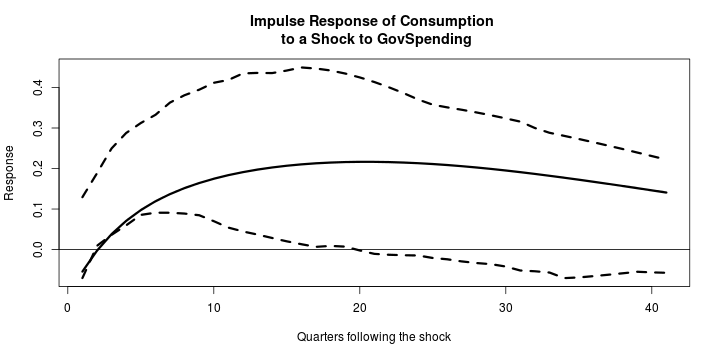
\includegraphics[scale=0.34]{pics/irf_sh_GovSpending_var_Consumption.png} & 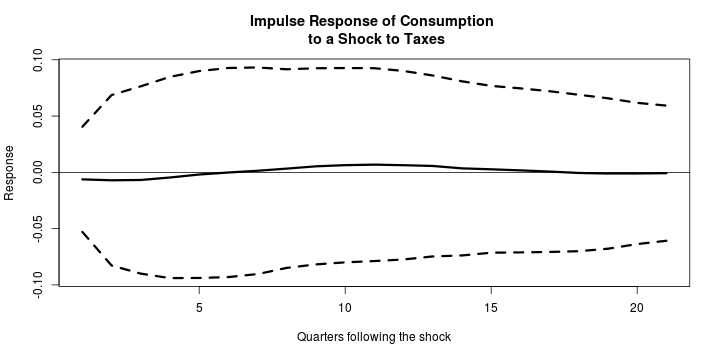
\includegraphics[scale=0.34]{pics/irf_sh_Taxes_var_Consumption.png} \\
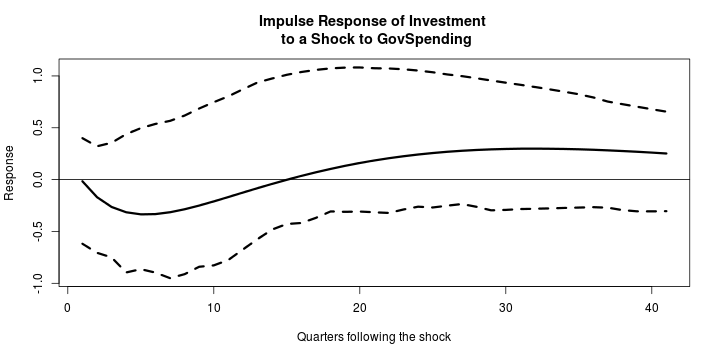
\includegraphics[scale=0.34]{pics/irf_sh_GovSpending_var_Investment.png} & 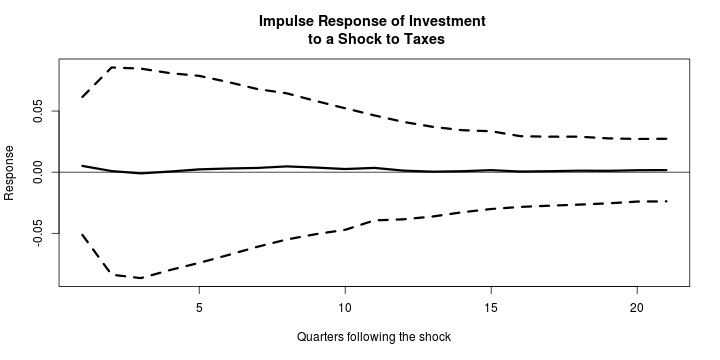
\includegraphics[scale=0.34]{pics/irf_sh_Taxes_var_Investment.png} \\
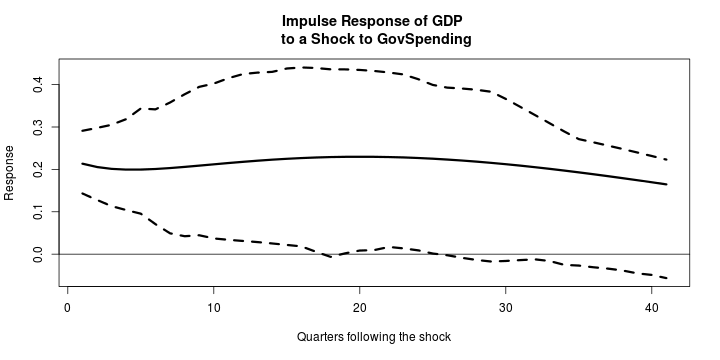
\includegraphics[scale=0.34]{pics/irf_sh_GovSpending_var_GDP.png} & 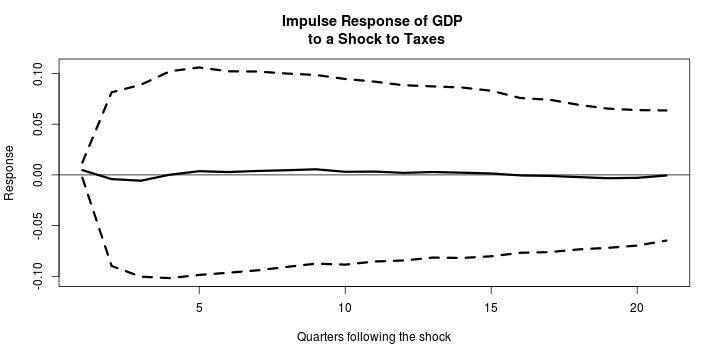
\includegraphics[scale=0.34]{pics/irf_sh_Taxes_var_GDP.png} \\
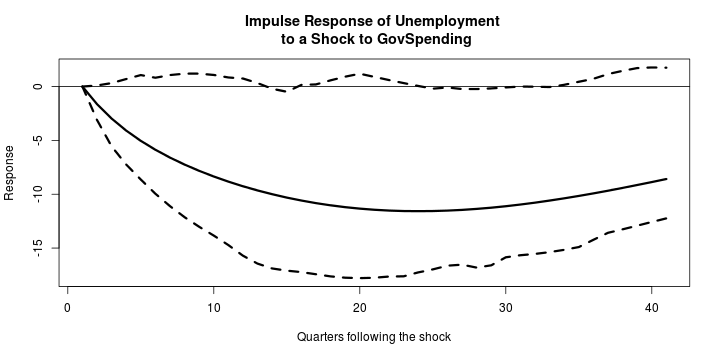
\includegraphics[scale=0.34]{pics/irf_sh_GovSpending_var_Unemployment.png} & 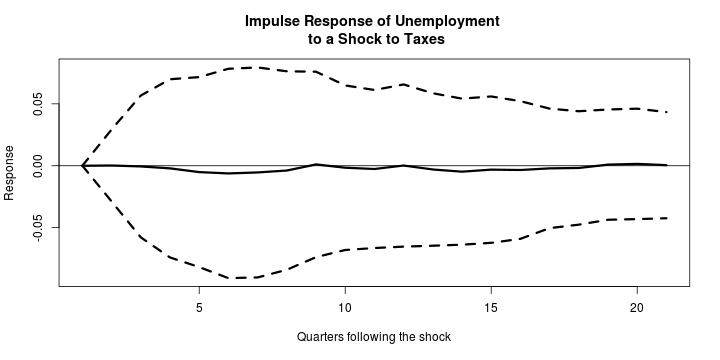
\includegraphics[scale=0.34]{pics/irf_sh_Taxes_var_Unemployment.png} 
\end{tabular}
\end{center}
\end{figure}

\begin{figure}\caption{Evolution of Expectations for Government Spending}\label{fg:exp_gov}
\begin{center}
\hspace*{-0.2in}\begin{tabular}{ccc}
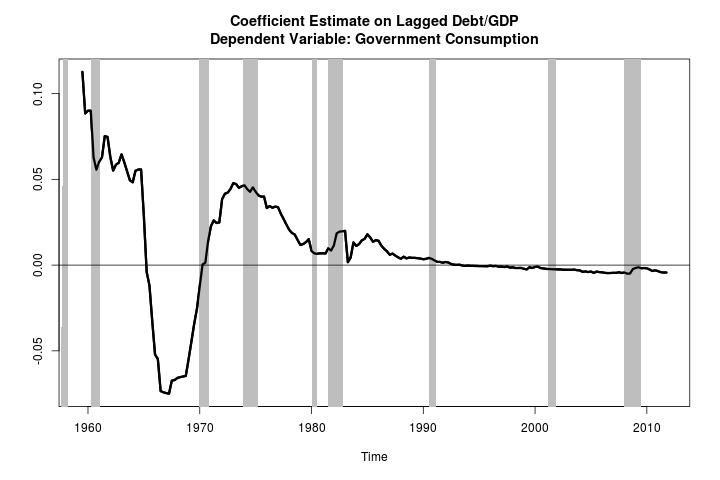
\includegraphics[scale=0.34]{pics/coef_govcons_debt.png} & 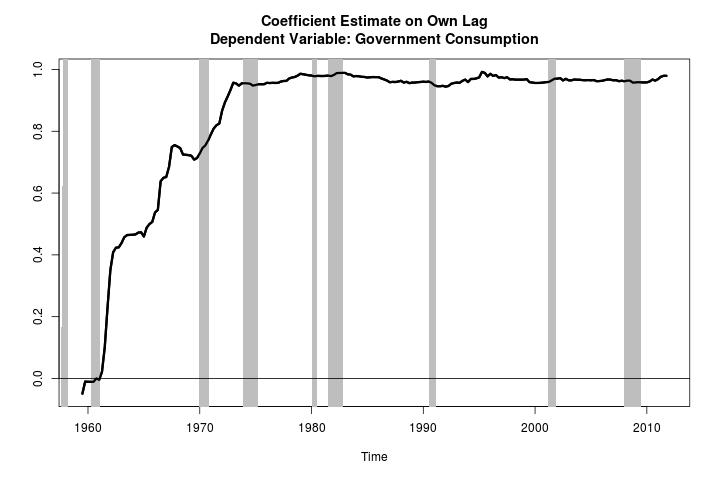
\includegraphics[scale=0.34]{pics/coef_govcons_lag.png} \\
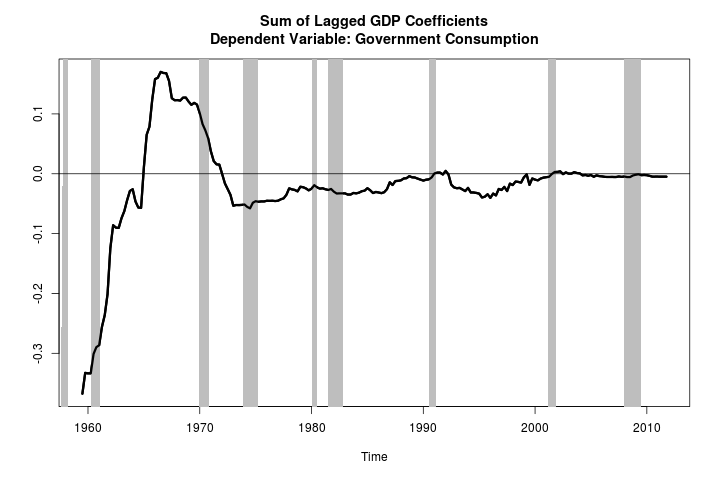
\includegraphics[scale=0.34]{pics/coef_govcons_gdp.png} & 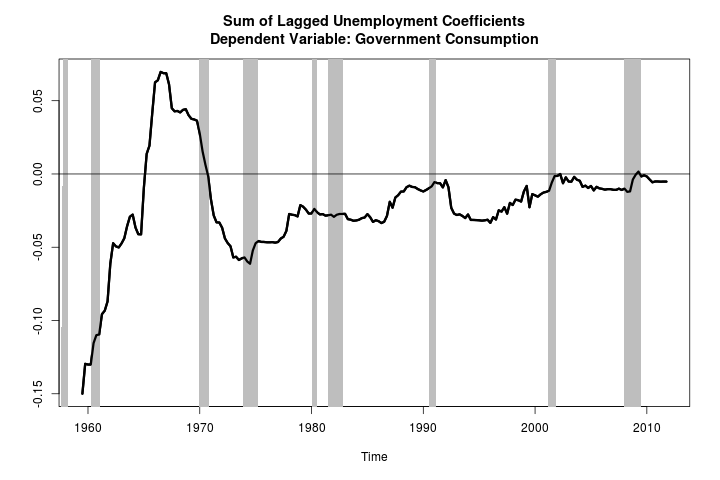
\includegraphics[scale=0.34]{pics/coef_govcons_unemployment.png} \\
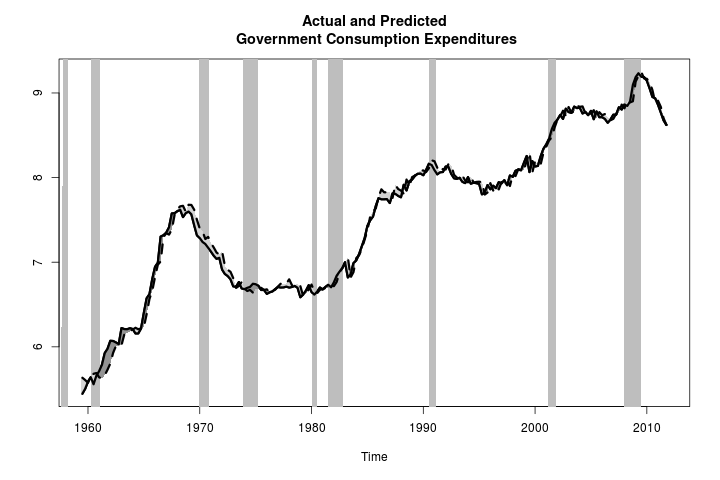
\includegraphics[scale=0.34]{pics/govcons.png} & 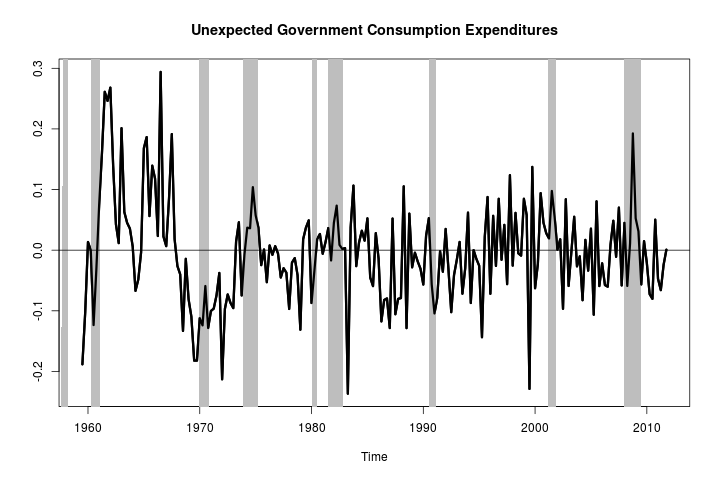
\includegraphics[scale=0.34]{pics/unexp_govcons.png}  \\ 
\end{tabular}
\end{center}
\end{figure}

\begin{figure}\caption{Evolution of Expectations for Net Taxes}\label{fg:exp_tax}
\begin{center}
\hspace*{-0.2in}\begin{tabular}{ccc}
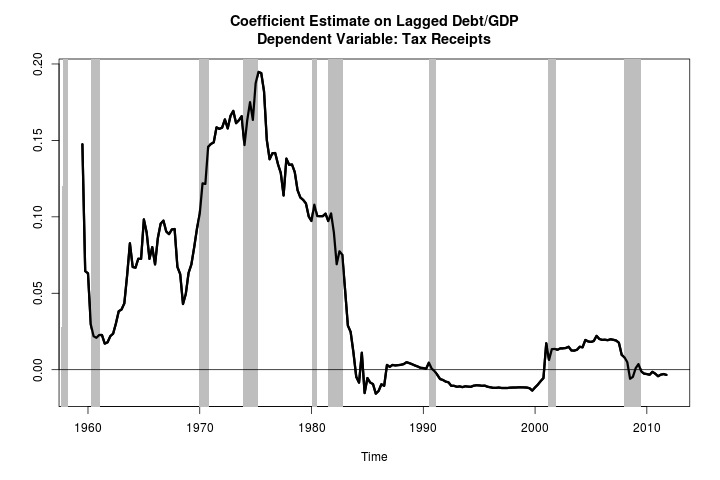
\includegraphics[scale=0.34]{pics/coef_tax_debt.png} & 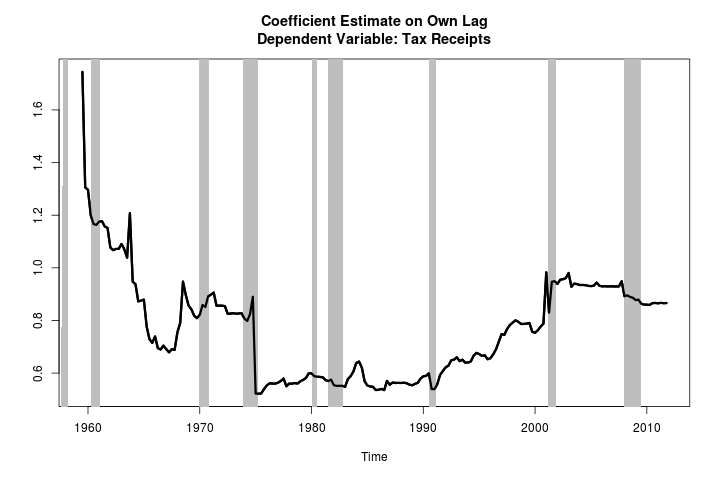
\includegraphics[scale=0.34]{pics/coef_tax_lag.png} \\
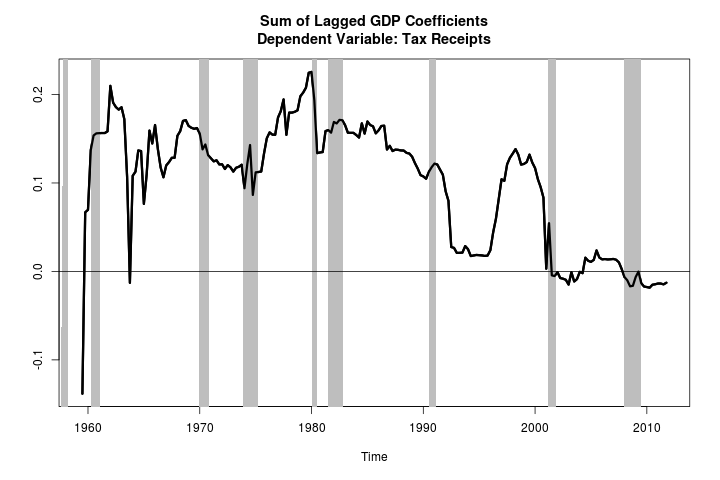
\includegraphics[scale=0.34]{pics/coef_tax_gdp.png} & 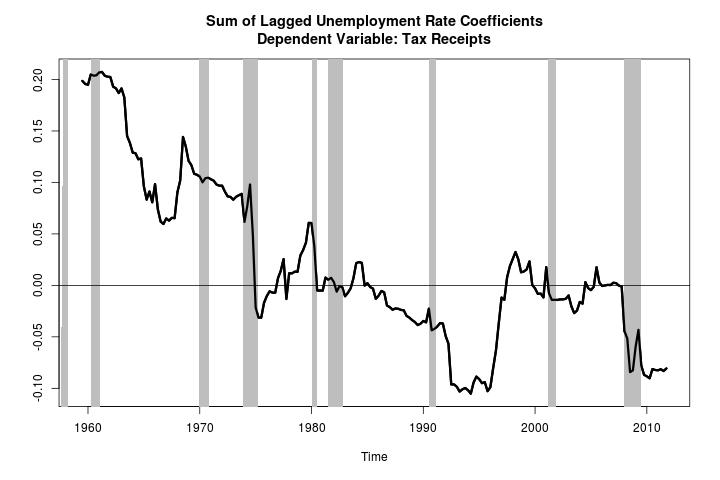
\includegraphics[scale=0.34]{pics/coef_tax_unemployment.png} \\
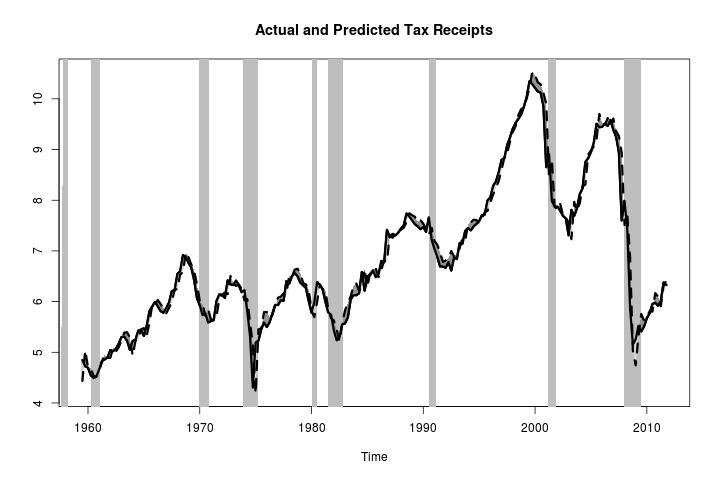
\includegraphics[scale=0.34]{pics/taxrev.png} & 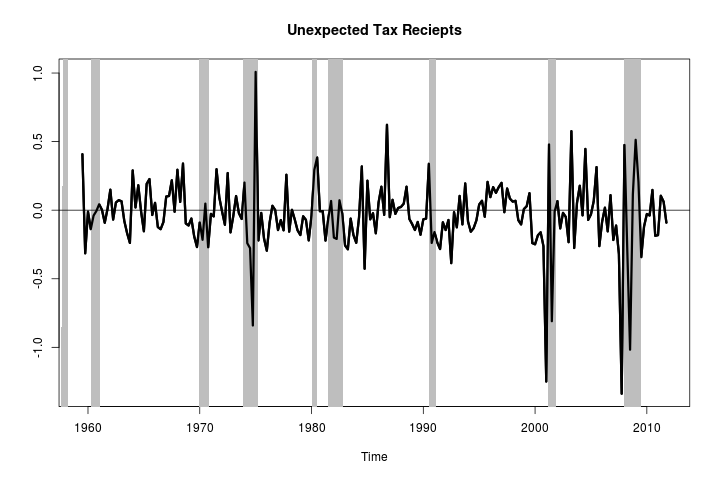
\includegraphics[scale=0.34]{pics/unexp_tax.png}  \\ 
\end{tabular}
\end{center}
\end{figure}


\begin{figure}\caption{Impulse Responses to Shocks in Expected and Unexpected Government Spending}\label{fg:irf_gov}
\begin{center}
\hspace*{-0.2in}\begin{tabular}{cc}
\includegraphics[scale=0.34]{pics/irf_sh_Predicted\space Government\space Spending_var_Consumption.png} & \includegraphics[scale=0.34]{pics/irf_sh_Unexpected\space Government\space Spending_var_Consumption.png} \\
\includegraphics[scale=0.34]{pics/irf_sh_Predicted\space Government\space Spending_var_Investment.png} & \includegraphics[scale=0.34]{pics/irf_sh_Unexpected\space Government\space Spending_var_Investment.png} \\
\includegraphics[scale=0.34]{pics/irf_sh_Predicted\space Government\space Spending_var_GDP.png} & \includegraphics[scale=0.34]{pics/irf_sh_Unexpected\space Government\space Spending_var_GDP.png} \\
\includegraphics[scale=0.34]{pics/irf_sh_Predicted\space Government\space Spending_var_Unemployment.png} & \includegraphics[scale=0.34]{pics/irf_sh_Unexpected\space Government\space Spending_var_Unemployment.png} 
\end{tabular}
\end{center}
\end{figure}

\begin{figure}\caption{Impulse Responses to Shocks in Expected and Unexpected Net Taxes}\label{fg:irf_tax}
\begin{center}
\hspace*{-0.2in}\begin{tabular}{cc}
\includegraphics[scale=0.34]{pics/irf_sh_Predicted\space Taxes_var_Consumption.png} & \includegraphics[scale=0.34]{pics/irf_sh_Unexpected\space Taxes_var_Consumption.png} \\
\includegraphics[scale=0.34]{pics/irf_sh_Predicted\space Taxes_var_Investment.png} & \includegraphics[scale=0.34]{pics/irf_sh_Unexpected\space Taxes_var_Investment.png} \\
\includegraphics[scale=0.34]{pics/irf_sh_Predicted\space Taxes_var_GDP.png} & \includegraphics[scale=0.34]{pics/irf_sh_Unexpected\space Taxes_var_GDP.png} \\
\includegraphics[scale=0.34]{pics/irf_sh_Predicted\space Taxes_var_Unemployment.png} & \includegraphics[scale=0.34]{pics/irf_sh_Unexpected\space Taxes_var_Unemployment.png} 
\end{tabular}
\end{center}
\end{figure}

\end{document}
